\documentclass[letterpaper,11pt]{article}
\usepackage[spanish]{babel}
\usepackage[utf8]{inputenc}
\usepackage{graphicx}
\DeclareGraphicsExtensions{.jpg,.pdf,.mps,.png}
%Paquetes adicionales, ayudan para portada (algunos)
\usepackage{amssymb}
\usepackage{amsfonts}
\usepackage{amsmath}
\usepackage{fancyhdr}
\usepackage{wrapfig}
\usepackage[dvipsnames]{xcolor}
\colorlet{LightRubineRed}{RubineRed!70!}%https://www.overleaf.com/learn/latex/Using_colours_in_LaTeX
\usepackage{multicol}
\usepackage{changepage}
\usepackage{float}
\usepackage{tcolorbox}
\usepackage{enumitem}
%https://tex.stackexchange.com/questions/455341/how-to-represent-the-shift-key
%https://tex.stackexchange.com/questions/176398/carriage-return-symbol-new-command
\usepackage{keystroke}
\usepackage{menukeys}
\usepackage{tabularx,ragged2e,booktabs,caption}
\definecolor{gray51}{rgb}{0.51,0.51,0.51}


% Márgenes
\usepackage[vmargin=1.5cm,hmargin=2cm,head=30pt,includeheadfoot]{geometry}

% Interlineado
\linespread{1.5}
\usepackage{hyperref}
\usepackage{natbib}
\setcitestyle{super}
\usepackage{blindtext}
\linespread{1.0}\selectfont

% Definir estilo fancy
% Encabezado
\fancypagestyle{style1}{
\fancyhf{}
\lhead{
  \begin{wrapfigure}{l}{0.2\textwidth}
    \vspace{-0.69cm}
    \noindent \hspace{-1.10cm} 
\includegraphics[scale=0.2]{logos_dcc/logo_fac/fcfm_dcc_png}
  \end{wrapfigure}
  \hspace*{0.3cm}
  \textcolor{RubineRed}{\textsf{Liceo 1 Javiera Carrera}} \\
  \hspace*{0.3cm}
  \textcolor{gray51}{\textsc{Resumen Probabilidad N$^{o}$1}}} % Licencia en la izquierda del encabezado
\rhead{} % Logo
\fancyfoot{}
\renewcommand{\headrulewidth}{0.4pt}
}


\fancypagestyle{style2}{
\fancyhf{}
\lhead{
\begin{wrapfigure}{l}{0.2\textwidth}
\vspace{-2.4cm}

\includegraphics[scale=0.2]{fcfm_dcc_png}
\end{wrapfigure}
  %\hspace*{0.3cm}
  %\textcolor{RubineRed}{\textsf{Liceo 1 Javiera Carrera}} \\
  %\hspace*{0.3cm}
  %\textcolor{gray51}{\textsc{Resumen Probabilidad N$^{o}$1}} % Licencia en la izquierda del encabezado
  %\vspace{0.6cm}
} % TITULO DEL ENSAYO
\rhead{\textsf{Universidad de Chile\\ Departamento de Ciencia de la Computación}\\
\textbf{\textsf{Modelacion y Comp. Gráfica CC3501}}
\vspace{0.1cm}}
\renewcommand{\headrulewidth}{0.4pt}
}


\begin{document}

\pagestyle{style2}
\begin{figure}
\centering
\begin{minipage}[c]{0.8\textwidth}
\centering
\vspace{0.3cm}
{\Large Informe de documentación}
\vspace{0.3cm}\\
Profesor: Daniel Calderón\\
Fecha: \today\\
Autor: Sebastián Sepúlveda A.
\end{minipage}
\end{figure}

\textbf{{\Large Solución del problema}}

Primero se realizó un análisis de los problemas principales que se deberian resolver, como la estructura de datos que se utilizaría (Estructura de árbol), creación de los objetos minimos pedidos (peces, algas, suelo, barco), aleatoridad de la posición de los pescados, la creación de nuevos pescados en distintos lugares a los ya creados, darle movimiento a los peces y a las burbujas con funciones utiles y finalmente, eliminar a los peces al hacer click sobre ellos.
\\

La primera etapa fue crear el escenario maritimo elaborando los objetos importantes y básicos, que serian de utilidad para hacer los elementos más complejos. Cuadrado, triangulo y circulo  fueron las figuras básicas que se utilizaron. En el proceso de crear a los elementos más complejos como el pescado, la alga y las burbujas, se ocupó el apoyo de la modelación jerárquica con árboles, y el apoyo de la libreria \texttt{scene graph} vista en clases. La finalidad de ocupar arboles, era aprovechar las funciones de la libreria y poder trabajar con cada objeto de manera independiente en la animación.
\\

La segunda etapa consistió en crear rocas, algas, peces, un barco naufrago y burbujas. Los dos elementos más complejos para su construcción fueron los peces, el barco y las algas. Para los peces se basó en la combinación de las tres figuras básicas, y se resolvió como crearlos de tal manera que su posición, color y escala fuera aleatorio (se utilizó la libreria \texttt{ramdom} de python). Mientras que para el barco y las algas, se ocuparon transformaciones y uso de figuras convenientes para mostrarlos más realistas.
\\

La tercera fue el proceso de animación del programa. En ella se hizo una animación a los peces y a las burbujas. El orden en la elaboración de este proceso era primordial para lograr que las transformaciones realizadas consecutivamente a cada pez creado y por crear o a las burbujas que permanecian estaticas, se lograran de la forma que se requeria, sin saltos, sin perdida de información de la posición, aleatoridad, etc. Para los peces se generaron movimientos en ZIG-ZAG, sinusoidales, parabolicos, rectos, etc. Mientras que para las burbujas, se creo un movimiento traslacional solamente. La forma de resolverlo fue añadirles movimiento a cada objeto después de haberlo creado, buscando el nodo correcto donde se realizaría la transformación.
\\

La cuarta y última etapa fue la interacción con el usuario. En esta etapa se pudo resolver fácilmente el añadir la tecla Enter para que el usuario pueda sumar peces cada vez que presiona. La eliminación de los peces se implementó con un recorrido en la lista de hijos del arbol que contiene a los peces, llamado \texttt{`` cardumen ''}, eliminando al pez que tenga la posición más cercana al hacer click en el mouse. Sin embargo, cuando se realizó el test, no se logran los resultados esperados, existiendo momentos en que los peces en los cuales se hace ``click'' siguen en pantalla, o se eliminan otros. La falla en este proceso puede deberse a una mala implementación y a errores en la redacción del código.
\\

\textbf{{ Dificultades:}}

Las etapas más dificiles de la implementación fueron la eliminación de los pescados y la animación de los movimientos en los objetos. El tiempo aproximado dedicado a estos problemas fue cercano a 6 horas, sumado a 3 commits importantes dedicados solamente a estas animaciones.
\\

\textbf{{ Instrucciones de ejecución:}}
\par

Para que aparezcan los peces es necesario hacer click en Enter \keys{\return}, y para que los peces desaparezcan es necesario presionar Click izquierdo sobre el pez, o algún punto en la ventana.
\\

\begin{minipage}[h]{\textwidth}
  \centering
  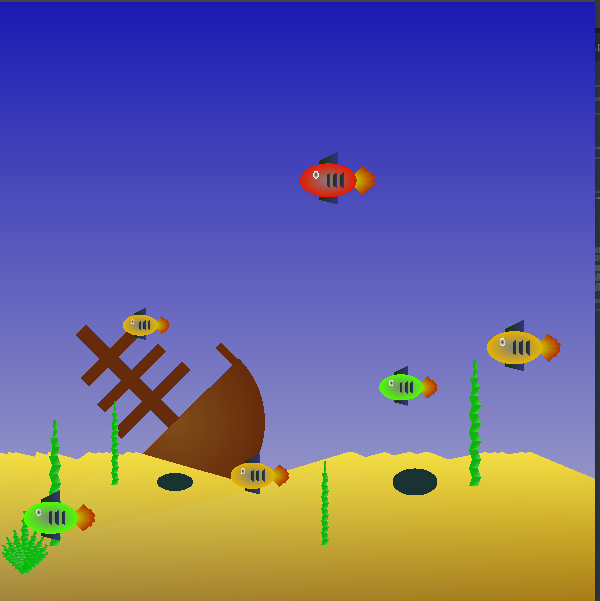
\includegraphics[scale=0.3]{images/tarea1/enter.png}
  \captionof{figure}{Escenario cuando están los peces en pantalla}
  \label{fig: pez1}
\end{minipage}

\begin{minipage}[h]{\textwidth}
  \centering
  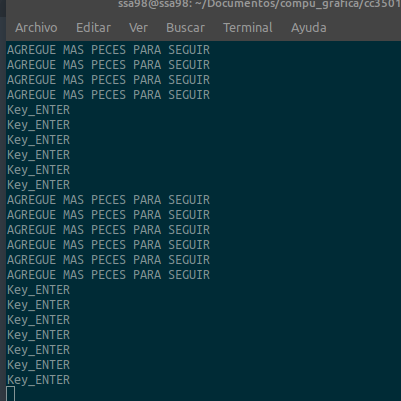
\includegraphics[scale=0.3]{images/tarea1/enter_comando.png}
  \captionof{figure}{Mensaje de salida al presionar enter o click izquierdo, dependiendo del caso}
  \label{fig: pez2}
\end{minipage}



\end{document}
